
\begin{appendices}

\chapter{Engelse gevoelsanalyse versus Nederlandse Gevoelsanalyse}\label{Naive Bayes Classifier met hetzelfde onderwerp voor trainings- en testset}
Algemeen voor alle experimenten zijn de resultaten berekend als gemiddelde over dertig runs. Dit wil zeggen dat er telkens bij iedere run een nieuwe Naive Bayes Classifier wordt aangemaakt en vervolgens getraind en getest wordt met een andere trainings- en testset als de andere runs. Om te verzekeren dat bij elke run de trainingsset en testset verschillend zijn wordt bij iedere run de trainingsset en testset aangemaakt  door een bepaald aantal willekeurig uit de grote pool van recensies te selecteren. Na het uitvoeren van die runs wordt hier het gemiddelde van genomen. De resultaten van experimenten bestaan uit de classificatieprecisie van zowel de trainings- als testset, de standaard afwijking, de confusion matrix en het betrouwbaarheidsinterval voor 95\%. Het betrouwbaarheidsinterval wordt als \textit{(gemiddeld ; linkerlimiet ; rechterlimiet)} genoteerd. Een 2 matrix geeft aan hoeveel van elke outputmogelijkheid er juist zijn ge\"identificeerd door de classifier en hoeveel er fout als juist zijn ge\"identificeerd. Als laatste wordt er ook de learning curve bekeken om over- of underfitting uit te sluiten. De learning curve geeft het verloop van de precisie van de classifier weer voor de trainings- en validatieset. Op basis van het verloop en de ligging van de curve kan men detecteren of men te maken heeft met over- of underfitting. Figuur \ref{fig:highbias} en \ref{fig:highvariance} illustreren hoe men overfitting kan herkennen aan de hand van de learning curve. Merk op zowel de trainingsset als de testset altijd evenwichtig zijn verdeeld. Dit wil zeggen dat er telkens 1/2 van het totaal aantal samples bestaat uit positieve recensies en 1/2 uit negatieve recensies.
\newpage
\begin{figure}[h]
    \centering
    \subfloat{{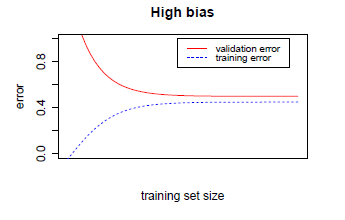
\includegraphics[width=5cm]{highbias}}}%
    \caption{Learning curve van een dataset met hoge bias. Wat duidt op underfitting [Bron: VUB-Cursus Machine Learning]}
    \label{fig:highbias}
 \end{figure}
 \begin{figure}[h]
 \centering
    \subfloat{{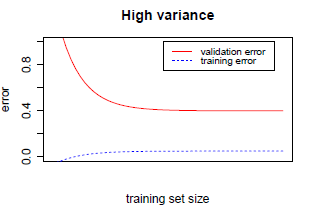
\includegraphics[width=5cm]{highvariance} }}%
    \caption{Learning curve van een dataset met hoge variantie. Wat duidt op overfitting [Bron: VUB-Cursus Machine Learning]}
    \label{fig:highvariance}
\end{figure}
\renewcommand\arraystretch{1.5}
\setlength\tabcolsep{0pt}
\begin{table}[h!]
\centering
\begin{tabular}{c >{\bfseries}r @{\hspace{0.7em}}c @{\hspace{0.4em}}c @{\hspace{0.7em}}l}
  \multirow{10}{*}{\parbox{1.1cm}{\bfseries\raggedleft eigelijke\\ waarde}} & 
    & \multicolumn{2}{c}{\bfseries voorspelde waarde} & \\
  & & \bfseries p & \bfseries n  \\
  & p$'$ & \MyBox{Waar}{Positief} & \MyBox{Vals}{Negatief}  \\[2.4em]
  & n$'$ & \MyBox{Vals}{Positief} & \MyBox{Waar}{Negatief} \\
\end{tabular}
\caption{Illustratie van de confusion matrix} 
\end{table}



\subsection{Filmrecensies als trainings- en testset}\label{Films als trainings- en testset}

Eerst trainen en testen we de Naive Bayes Classifier met filmrecensies. De trainingsset bestaat uit 6000 samples en de testset uit 2000 samples. Zoals eerder vermeld werden deze samples at random geselecteerd en is het volgende resultaat het gemiddelde van 30 runs.\\

\newpage\textbf{Standaard afwijking} = 0,0094\\
\textbf{95\% betrouwbaarheidsinterval} = (0,7064 ; 0,7030 ; 0,7101)\\

\begin{table}[h]
\centering
\setlength\tabcolsep{4pt}
\begin{minipage}[t]{0.48\textwidth}
\centering
\begin{tabular}{l|l|}
\cline{2-2}
                                            & \textbf{Precisie} \\ \hline
\multicolumn{1}{|l|}{\textbf{Trainingsset}} & 90,52\%           \\ \hline
\multicolumn{1}{|l|}{\textbf{Testset}}      & 70,66\%           \\ \hline
\end{tabular}
\caption{Classificatieprecisie Naive Bayes Classifier, getraind op filmrecensies}
\label{tab:movie-movie}
\end{minipage}%
\hfill
\begin{minipage}[t]{0.48\textwidth}
\centering
\begin{tabular}{lll}
                                 & \textbf{P}               & \textbf{N}               \\ \cline{2-3} 
\multicolumn{1}{l|}{\textbf{P'}} & \multicolumn{1}{l|}{824} & \multicolumn{1}{l|}{175} \\ \cline{2-3} 
\multicolumn{1}{l|}{\textbf{N'}} & \multicolumn{1}{l|}{410} & \multicolumn{1}{l|}{589} \\ \cline{2-3} 
\end{tabular}
\caption{Confusion matrix van de testset door de  Naive Bayes Classifier, getraind op filmrecensies} 
\label{tab:cm-movie-movie} 
\end{minipage}
\end{table}

Zoals men kan zien aan de resultaten zijn de prestaties goed. Een classificatieprecisie van 70\% voor een onbekende set met filmrecensies is een goede prestatie. Verder is het betrouwbaarheidsinterval heel klein, wat maakt dat we met 95\% kunnen zeggen dat de classificatie van filmrecensies door een Naive Baiyes Classifier, getraind op filmrecensies, met een precisie tussen 70\% en 71\% gebeurd. De confusion matrix geeft ons  ook een inzicht in wat er juist en fout geclassificeerd is. We zien dat de classifier overwegend beter positieve recensies kan identificeren dan negatieve.\\
%
Ten slotte wat we ook kunnen afleiden uit de cijfers, waar we zien dat zowel de test- als trainingsset goed presteren, zien we aan de learning curve dat we geen over- of underfitting hebben. 

\begin{figure}[h]%
    \centering
    \subfloat{{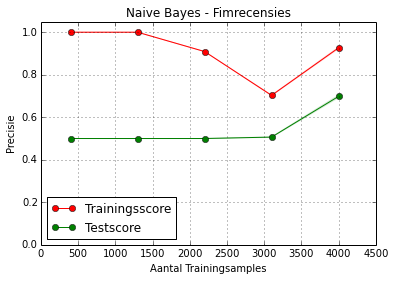
\includegraphics[width=5cm]{lc-movie-movie}}}%
    \label{fig:lc-movie-movie}
    \caption{Learning curve van de training van de Naive Bayes Classifier op filmrecensies}
\end{figure}

\subsection{Muziekrecensies als trainings- en testset}\label{Muziek als trainings- en testset}

Nu trainen en testen we de Naive Bayes Classifier met muziekrecensie. De trainingsset bestaat uit 6000 samples en de testset uit 2000 samples. Wederom werden deze samples at random geselecteerd en is het volgende resultaat het gemiddelde van 30 runs.\\

\textbf{Standaard afwijking} = 0,0096\\
\textbf{95\% betrouwbaarheidsinterval} = (0,8262 ; 0,8226 ; 0,8299)\\
 
\begin{table}[h]
\centering
\setlength\tabcolsep{4pt}
\begin{minipage}[t]{0.48\textwidth}
\centering
\begin{tabular}{l|l|}
\cline{2-2}
                                            & \textbf{Precisie} \\ \hline
\multicolumn{1}{|l|}{\textbf{Trainingsset}} & 93,44\%           \\ \hline
\multicolumn{1}{|l|}{\textbf{Testset}}      & 82,62\%           \\ \hline
\end{tabular}
\caption{Classificatieprecisie Naive Bayes Classifier, getraind op muziekrecensies}
\end{minipage}%
\hfill
\begin{minipage}[t]{0.48\textwidth}
\centering
\begin{tabular}{lll}
                                 & \textbf{P}               & \textbf{N}               \\ \cline{2-3} 
\multicolumn{1}{l|}{\textbf{P'}} & \multicolumn{1}{l|}{879} & \multicolumn{1}{l|}{120} \\ \cline{2-3} 
\multicolumn{1}{l|}{\textbf{N'}} & \multicolumn{1}{l|}{227} & \multicolumn{1}{l|}{772} \\ \cline{2-3} 
\end{tabular}
\caption{Confusion matrix van de testset door de  Naive Bayes Classifier, getraind op muziekrecensies} 
\end{minipage}
\end{table}

Hier zien we eveneens goede resultaten. Een classificatieprecisie van 82\% voor een onbekende set met muziekrecensies is eveneens een goede prestatie. Wederom is het betrouwbaarheidsinterval heel klein, wat maakt dat we met 95\% kunnen zeggen dat de classificatie van muziekrecensies door een Naive Baiyes Classifier, getraind op muziekrecensies, met een precisie van 82\% gebeurd. De confusion matrix toont ons opnieuw dat de classifier beter om kan met positieve recensies.
%
Wederom geeft onderstaande learning curve uitsluiting van over- of underfitting .

\begin{figure}[h]%
    \centering
    \subfloat{{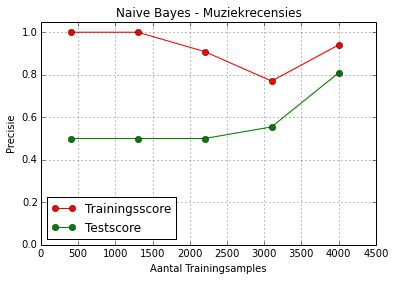
\includegraphics[width=5cm]{lc-music-music}}}%
    \label{fig:lc-music-music}
    \caption{Learning curve van de training van de Naive Bayes Classifier op muziekrecensies}
\end{figure}

\subsection{Boekrecensies als trainings- en testset}\label{Boeken als trainings- en testset}

Als laatste trainen en testen we de Naive Bayes Classifier met boekrecensies. De trainingsset bestaat uit 218 samples en de testset uit 74 samples. De samples zijn wederom at random geselecteerd en het resultaat is het gemiddelde van 30 runs.\\

\textbf{Standaard afwijking} = 0,0640\\
\textbf{95\% betrouwbaarheidsinterval} = (0,7176 ; 0,6932 ; 0,7419)\\
 
\begin{table}[h]
\centering
\setlength\tabcolsep{4pt}
\begin{minipage}[t]{0.48\textwidth}
\centering
\begin{tabular}{l|l|}
\cline{2-2}
                                            & \textbf{Precisie} \\ \hline
\multicolumn{1}{|l|}{\textbf{Trainingsset}} & 99,43\%           \\ \hline
\multicolumn{1}{|l|}{\textbf{Testset}}      & 71,76\%           \\ \hline
\end{tabular}
\caption{Classificatieprecisie Naive Bayes Classifier, getraind op boekrecensies}
\end{minipage}%
\hfill
\begin{minipage}[t]{0.48\textwidth}
\centering
\begin{tabular}{lll}
                                 & \textbf{P}               & \textbf{N}            \\ \cline{2-3} 
\multicolumn{1}{l|}{\textbf{P'}} & \multicolumn{1}{l|}{31} & \multicolumn{1}{l|}{5} \\ \cline{2-3} 
\multicolumn{1}{l|}{\textbf{N'}} & \multicolumn{1}{l|}{15} & \multicolumn{1}{l|}{21} \\ \cline{2-3} 
\end{tabular}
\caption{Confusion matrix van de testset door de  Naive Bayes Classifier, getraind op boekrecensies} 
\end{minipage}
\end{table}


Hier zien we ook goede resultaten. Een classificatieprecisie van 72\% voor een onbekende set met boekrecensies is een eveneens een goede prestatie. Hier zien we wel dat het betrouwbaarheidsinterval ruimer en is met 95\% zekerheid te zeggen, dat de classificatieprecisie zich tussen de 69\% en 74\% situeert, wat nog altijd acceptabel is. De confusion matrix toont ons opnieuw dat de classifier beter om kan met positieve recensies, al valt dit te nuanceren, aangezien we maar een hele klein pool hebben aan boekrecensies ten opzichte van de rest. Onderstaande learning curve sluit opnieuw over- en underfitting uit.\\
\newpage
\begin{figure}%
    \centering
    \subfloat{{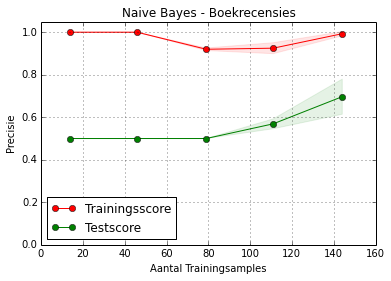
\includegraphics[width=5cm]{lc-boek-boek}}}%
    \label{fig:lc-boek-boek}
    \caption{Learning curve van de training van de Naive Bayes Classifier op boekrecensies}
\end{figure}

Nu we de prestaties weten van de Naive Bayes classifier met als trainings- en testset hetzelfde onderwerp. Kunnen we eens kijken wat de prestaties zijn met een verschillend onderwerp voor de trainingsset en testset.  

\section{Naive Bayes Classifier met een verschillend onderwerp voor trainings- en testset}\label{Naive Bayes Classifier met verschillend onderwerp voor trainings- en testset}

In \ref{Naive Bayes Classifier met hetzelfde onderwerp voor trainings- en testset} zagen we al dat de classificatie met een Naive Bayes Classifier, waarbij trainings- en testset tot hetzelfde onderwerp behoren, goede resultaten oplevert. Nu gaan we kijken of dit ook het geval is wanneer trainingsset en testset verschillend zijn. Wederom alle samples worden at random geselecteerd en de resultaten weerspiegelen telkens het gemiddelde van 30 runs.  

\subsection{Filmrecensies als trainingsset}\label{Filmrecensies als trainingsset}

Als eerste nemen we een getrainde Naive Bayes Classifier op filmrecensies en bekijken we de resultaten op een testset van muziek- en boekrecensies. De Naive Bayes Classifier is telkens getraind met 6000 samples.

\subsubsection{Muziekrecensies als testset}\label{Muziekrecensies als testset-movie}

De testset bestaat uit 2000 samples waarvan 1/2 positieve en 1/2 negatieve recensies.\\

\textbf{Standaard afwijking} = 0,01467\\
\textbf{95\% betrouwbaarheidsinterval} = (0,6207 ; 0,6152 ; 0,6263)\\
 
\begin{table}[h]
\centering
\setlength\tabcolsep{4pt}
\begin{minipage}[t]{0.48\textwidth}
\centering
\begin{tabular}{l|l|}
\cline{2-2}
                                            & \textbf{Precisie} \\ \hline
\multicolumn{1}{|l|}{\textbf{Testset}}      & 62,07\%           \\ \hline
\end{tabular}
\caption{Classificatieprecisie Naive Bayes Classifier, getraind op filmrecensies, getest op muziekrecensies}
\end{minipage}%
\hfill
\begin{minipage}[t]{0.48\textwidth}
\centering
\begin{tabular}{lll}
                                 & \textbf{P}               & \textbf{N}               \\ \cline{2-3} 
\multicolumn{1}{l|}{\textbf{P'}} & \multicolumn{1}{l|}{655} & \multicolumn{1}{l|}{345} \\ \cline{2-3} 
\multicolumn{1}{l|}{\textbf{N'}} & \multicolumn{1}{l|}{413} & \multicolumn{1}{l|}{586} \\ \cline{2-3} 
\end{tabular}
\caption{Confusion matrix van de testset ,bestaande uit muziekrecensies, door de  Naive Bayes Classifier, getraind op filmrecensies} 
\end{minipage}
\end{table}

De prestatie is minder dan de prestaties in \ref{Naive Bayes Classifier met hetzelfde onderwerp voor trainings- en testset}, maar 62\% is zeker aanvaardbaar. Ook het betrouwbaarheidsinterval is klein wat wil zeggen dat we  met 95\% zekerheid kunnen zeggen dat een Naive Bayes Classifier getraind op filmrecensies, muziekrecensies net 61\%-62\% precisie kan classificeren.  

\subsubsection{Boekrecensies als testset}\label{Boekrecensies testset-movie}

De testset bestaat uit 146 samples waarvan 1/2 positief en 1/2 negatief.\\

\textbf{Standaard afwijking} = 0,03714\\
\textbf{95\% betrouwbaarheidsinterval} = (0,6586 ; 0,6446 ; 0,6728)\\
 
\begin{table}[h]
\centering
\setlength\tabcolsep{4pt}
\begin{minipage}[t]{0.48\textwidth}
\centering
\begin{tabular}{l|l|}
\cline{2-2}
                                            & \textbf{Precisie} \\ \hline
\multicolumn{1}{|l|}{\textbf{Testset}}      & 65,87\%           \\ \hline
\end{tabular}
\caption{Classificatieprecisie Naive Bayes Classifier, getraind op filmrecensies, getest op boekrecensies}
\end{minipage}%
\hfill
\begin{minipage}[t]{0.48\textwidth}
\centering
\begin{tabular}{lll}
                                 & \textbf{P}               & \textbf{N}               \\ \cline{2-3} 
\multicolumn{1}{l|}{\textbf{P'}} & \multicolumn{1}{l|}{54} & \multicolumn{1}{l|}{18} \\ \cline{2-3} 
\multicolumn{1}{l|}{\textbf{N'}} & \multicolumn{1}{l|}{31} & \multicolumn{1}{l|}{41} \\ \cline{2-3} 
\end{tabular}
\caption{Confusion matrix van de testset, bestaande uit boekrecensies, door de  Naive Bayes Classifier, getraind op filmrecensies} 
\end{minipage}
\end{table}

De prestatie is in dezelfde lijn als de resultaten bij muziek. 

\subsection{Muziekrecensies als trainingsset}\label{Muziekrecensies als trainingsset}

Als tweede nemen we een getrainde Naive Bayes Classifier op muziekrecensies en bekijken we de resultaten op een testset van film- en boekrecensies. De Naive Bayes Classifier is telkens getraind met 6000 samples.

\subsubsection{Filmrecensies als testset}\label{Filmrecensies als testset}

De testset bestaat uit 2000 samples waarvan 1/2 positief en 1/2 negatief.\\

\textbf{Standaard afwijking} = 0,01146\\
\textbf{95\% betrouwbaarheidsinterval} = (0,6107 ; 0,6063 ; 0,6150)
 
\begin{table}[h]
\centering
\setlength\tabcolsep{4pt}
\begin{minipage}[t]{0.48\textwidth}
\centering
\begin{tabular}{l|l|}
\cline{2-2}
                                            & \textbf{Precisie} \\ \hline
\multicolumn{1}{|l|}{\textbf{Testset}}      & 61,07\%           \\ \hline
\end{tabular}
\caption{Classificatieprecisie Naive Bayes Classifier, getraind op muziekrecensies, getest op filmrecensies}
\end{minipage}%
\hfill
\begin{minipage}[t]{0.48\textwidth}
\centering
\begin{tabular}{lll}
                                 & \textbf{P}               & \textbf{N}               \\ \cline{2-3} 
\multicolumn{1}{l|}{\textbf{P'}} & \multicolumn{1}{l|}{691} & \multicolumn{1}{l|}{308} \\ \cline{2-3} 
\multicolumn{1}{l|}{\textbf{N'}} & \multicolumn{1}{l|}{469} & \multicolumn{1}{l|}{530} \\ \cline{2-3} 
\end{tabular}
\caption{Confusion matrix van de testset ,bestaande uit filmrecensies, door de  Naive Bayes Classifier, getraind op muziekrecensies} 
\end{minipage}
\end{table}

De resultaten zijn aanvaardbaar met een classificatieprecisie van 61\% en een klein betrouwbaarheidsinterval van 95\%.

\subsubsection{Boekrecensies als testset}\label{Boekrecensies als testset}

De testset bestaat uit 146 samples waarvan 1/2 positief en 1/2 negatief.\\

\textbf{Standaard afwijking} = 0,03519\\
\textbf{95\% betrouwbaarheidsinterval} = (0,6146 ; 0,6012 ; 0,6280)
 
\begin{table}[h]
\centering
\setlength\tabcolsep{4pt}
\begin{minipage}[t]{0.48\textwidth}
\centering
\begin{tabular}{l|l|}
\cline{2-2}
                                            & \textbf{Precisie} \\ \hline
\multicolumn{1}{|l|}{\textbf{Testset}}      & 61,46\%           \\ \hline
\end{tabular}
\caption{Classificatieprecisie Naive Bayes Classifier, getraind op muziekrecensies, getest op boekrecensies}
\end{minipage}%
\hfill
\begin{minipage}[t]{0.48\textwidth}
\centering
\begin{tabular}{lll}
                                 & \textbf{P}               & \textbf{N}               \\ \cline{2-3} 
\multicolumn{1}{l|}{\textbf{P'}} & \multicolumn{1}{l|}{43} & \multicolumn{1}{l|}{29} \\ \cline{2-3} 
\multicolumn{1}{l|}{\textbf{N'}} & \multicolumn{1}{l|}{26} & \multicolumn{1}{l|}{46} \\ \cline{2-3} 
\end{tabular}
\caption{Confusion matrix van de testset, bestaande uit boekrecensies, door de  Naive Bayes Classifier, getraind op muziekrecensies} 
\end{minipage}
\end{table}


Een gelijkaardige prestatie als filmrecensies, met een gemiddelde classificatieprecisie van 61\% en eveneens een klein betrouwbaarheidsinterval van 95\%.

\subsection{Boekrecensies als trainingsset}\label{Boekrecensies als trainingsset}

Als laatste nemen we een getrainde Naive Bayes Classifier op boekrecensies en bekijken we de resultaten op een testset van film- en muziekrecensies. De Naive Bayes Classifier is telkens getraind met 276 samples.


\subsubsection{Filmrecensies als testset}\label{Filmrecensies als testset}

De testset bestaat uit 2000 samples waarvan 1/2 positief en 1/2 negatief.\\

\textbf{Standaard afwijking} = 0,01812\\
\textbf{95\% betrouwbaarheidsinterval} = (0,5625 ; 0,5556 ; 0,5693)
 
\begin{table}[h]
\centering
\setlength\tabcolsep{4pt}
\begin{minipage}[t]{0.48\textwidth}
\centering
\begin{tabular}{l|l|}
\cline{2-2}
                                            & \textbf{Precisie} \\ \hline
\multicolumn{1}{|l|}{\textbf{Testset}}      & 56,25\%           \\ \hline
\end{tabular}
\caption{Classificatieprecisie Naive Bayes Classifier, getraind op boekrecensies, getest op filmrecensies}
\end{minipage}%
\hfill
\begin{minipage}[t]{0.48\textwidth}
\centering
\begin{tabular}{lll}
                                 & \textbf{P}               & \textbf{N}               \\ \cline{2-3} 
\multicolumn{1}{l|}{\textbf{P'}} & \multicolumn{1}{l|}{539} & \multicolumn{1}{l|}{460} \\ \cline{2-3} 
\multicolumn{1}{l|}{\textbf{N'}} & \multicolumn{1}{l|}{414} & \multicolumn{1}{l|}{585} \\ \cline{2-3} 
\end{tabular}
\caption{Confusion matrix van de testset ,bestaande uit filmrecensies, door de  Naive Bayes Classifier, getraind op boekrecensies} 
\end{minipage}
\end{table}

Met 56\% kunnen we spreken van een slechte prestatie. Net iets meer dan de helft van de classificaties wordt juist geclassificeerd. Het betrouwbaarheidsinterval is ook klein, wat betekent dat we met 95\% zekerheid kunnen zeggen dat de classificatieprecisie zich tussen 56\% - 57\% situeert. Wat nogmaals de slechte prestatie bevestigd.

\subsubsection{Muziekrecensies als testset}\label{Muziekrecensies als testset}

De testset bestaat uit 2000 samples waarvan 1/2 positief en 1/2 negatief.\\
\textbf{Standaard afwijking} = 0,01448\\
\textbf{95\% betrouwbaarheidsinterval} = (0,5647 ; 0,5592, 0,5702)

\begin{table}[h]
\centering
\setlength\tabcolsep{4pt}
\begin{minipage}[t!]{0.48\textwidth}
\centering
\begin{tabular}{l|l|}
\cline{2-2}
                                            & \textbf{Precisie} \\ \hline
\multicolumn{1}{|l|}{\textbf{Testset}}      & 56,47\%           \\ \hline
\end{tabular}
\caption{Classificatieprecisie Naive Bayes Classifier, getraind op boekrecensies, getest op muziekrecensies}
\end{minipage}%
\hfill
\begin{minipage}[t!]{0.48\textwidth}
\centering
\begin{tabular}{lll}
                                 & \textbf{P}               & \textbf{N}               \\ \cline{2-3} 
\multicolumn{1}{l|}{\textbf{P'}} & \multicolumn{1}{l|}{604} & \multicolumn{1}{l|}{395} \\ \cline{2-3} 
\multicolumn{1}{l|}{\textbf{N'}} & \multicolumn{1}{l|}{475} & \multicolumn{1}{l|}{524} \\ \cline{2-3} 
\end{tabular}
\caption{Confusion matrix van de testset, bestaande uit muziekrecensies, door de  Naive Bayes Classifier, getraind op boekrecensies} 
\end{minipage}
\end{table}

Een classificatieprecisie van 56\% is niet goed. Dit is analoog als bij voorgaande sectie met als testset filmrecensies\\

De resultaten op muziek- en filmrecensies zijn met 56\%, minder als de vorige in \ref{Filmrecensies als trainingsset} en \ref{Muziekrecensies als testset}, waar we rond de 60\% liggen.

\section{Conclusie experiment}\label{Conclusie experiment}

Nu we alle mogelijke combinaties van training en testing hebben uitgevoerd is het interessant om alle resultaten naast elkaar te leggen. Onderstaande tabel geeft nog eens alle classificatiescores in een kruistabel weer.

\begin{table}[h]
\centering
\begin{tabular}{l|c|c|c|}
\cline{2-4}
                                      & \textbf{Films} & \textbf{Muziek} & \textbf{Boeken} \\ \hline
\multicolumn{1}{|l|}{\textbf{Films}} & 70,66\%         & 61,00\%         & 56,25\%         \\ \hline
\multicolumn{1}{|l|}{\textbf{Muziek}} & 62,07\%         & 82,62\%         & 56,47\%         \\ \hline
\multicolumn{1}{|l|}{\textbf{Boeken}} & 65,87\%         & 61,46\%         & 71,76\%         \\ \hline
\end{tabular}
\label{tab:alles}
\caption{Kruistabel van alle classificatieresultaten uit \ref{Naive Bayes Classifier met verschillend onderwerp voor trainings- en testset} en \ref{Naive Bayes Classifier met hetzelfde onderwerp voor trainings- en testset} met de kolommen het onderwerp van de trainingsset en de rijen het onderwerp van de testset.} 
\end{table}


Op basis van de tabel kunnen we zeggen dat het trainen en testen met het zelfde onderwerp het beste resultaat geeft. Verder presteren muziek en films goed op een vreemde testset. Hierbij bedoelen we een testset die over een andere onderwerp gaat dan waar het algoritme op getraind is.  Boeken presteren hier minder. Dit kan te wijten zijn aan de kleinere dataset, waardoor er een bias of voorkeur ontstaat op bijvoorbeeld auteursnamen. Die bias op auteursnamen kan helpen bij het classificeren van boeken om positieve of negatieve recensies te herkennen, maar gaat niet helpen in de classificatie van een set over een ander onderwerp. Ook de prestatie van muziek springt in het oog met meer dan 10\% verschil tussen de andere classifiers met de trainingsset en testset over hetzelfde onderwerp. Maar het daalt wel 20\% wanneer het een vreemde set moet classificeren. Dit duidt eveneens op een bias of voorkeur op een bepaald feature die specifiek is voor muziek waardoor het classificeren van muziekrecensies veel beter gaat. Nog een interessant inzicht is dat filmrecensies een goede trainingsset blijken te zijn voor boekrecensies.  Ondanks de kleine dataset van boeken, kunnen we toch aan de hand van het betrouwbaarheidsinterval met 95\% zekerheid zeggen dat een getrainde Naive Bayes Classifier op filmrecensies, boekrecensies met een precisie tussen de 64\% en 67\% zal classificeren.\\

Nog een andere manier om de resultaten bij elkaar te leggen, is het bekijken van de confusion matrixen. We kunnen hier een percentueel gemiddelde van nemen en kijken hoe gemiddeld de classificatie verloopt bij sectie \ref{Naive Bayes Classifier met hetzelfde onderwerp voor trainings- en testset} waar de sets over hetzelfde onderwerp zijn en sectie \ref{Naive Bayes Classifier met verschillend onderwerp voor trainings- en testset}, waar ze verschillend zijn.

\begin{table}[h]
\centering
\setlength\tabcolsep{4pt}
\begin{minipage}[t]{0.48\textwidth}
\centering
\begin{tabular}{lll}
                                 & \textbf{P}               & \textbf{N}               \\ \cline{2-3} 
\multicolumn{1}{l|}{\textbf{P'}} & \multicolumn{1}{l|}{43\%} & \multicolumn{1}{l|}{6\%} \\ \cline{2-3} 
\multicolumn{1}{l|}{\textbf{N'}} & \multicolumn{1}{l|}{18\%} & \multicolumn{1}{l|}{31\%} \\ \cline{2-3} 
\end{tabular}
\caption{Gemiddelde confusion matrix in percent voor een Naive Bayes Classifier, waar trainings- en testset over hetzelfde onderwerp gaan}
\end{minipage}%
\hfill
\begin{minipage}[t]{0.48\textwidth}
\centering
\begin{tabular}{lll}
                                 & \textbf{P}               & \textbf{N}               \\ \cline{2-3} 
\multicolumn{1}{l|}{\textbf{P'}} & \multicolumn{1}{l|}{32\%} & \multicolumn{1}{l|}{18\%} \\ \cline{2-3} 
\multicolumn{1}{l|}{\textbf{N'}} & \multicolumn{1}{l|}{21\%} & \multicolumn{1}{l|}{29\%} \\ \cline{2-3} 
\end{tabular}
\caption{Gemiddelde confusion matrix in percent voor een Naive Bayes Classifier, waar trainings- en testset over een verschillend onderwerp gaan} 
\end{minipage}
\end{table}


Voor beide matrixen, ziet men duidelijk dat positieve recensies beter ge\"identificeerd worden. Na het herbekijken van de datasets, is een mogelijk verklaring dat mensen zich bij een positieve recensie zich veel expressiever en uitgebreider uitdrukken dan bij een negatieve recensie. Hierdoor krijgt de classifier meer informatie over de features van een positief document waardoor het beter het concept ``Positief'' kan bepalen 





%tabel klein experiment term weighting 
\begin{table}[]
\centering
\caption{My caption}
\label{my-label}
\begin{tabu} to \textwidth {|X|X|}
\hline
{\bf Recensie}                                                                                                                                                                                                                                                                                                                                                                                                                                                                                                                                                                                                                                                                                                                                                                                                                                                                                                                                                                                                                                                                                                                                                                                                                                                                                                                                                                                                                                                                                  & {\bf Woord met hoogste tf-idf score} \\ \hline
in het begin dacht ik echt van.. wat is dit nou weer.. maar je wil hem PERSE afzien! kei mooie film!aanrader!                                                                                                                                                                                                                                                                                                                                                                                                                                                                                                                                                                                                                                                                                                                                                                                                                                                                                                                                                                                                                                                                                                                                                                                                                                                                                                                                                                                   & Kei                                  \\ \hline
Geweldig verhaal! Aangrijpend. Ik heb deze film een stuk of 4 keer gezien, blijft indrukwekkend.****-sterren                                                                                                                                                                                                                                                                                                                                                                                                                                                                                                                                                                                                                                                                                                                                                                                                                                                                                                                                                                                                                                                                                                                                                                                                                                                                                                                                                                                    & Aangrijpend                          \\ \hline
Wat een geweldige film. De trilogy al 100 x gezien en het blijft goed. Ook vooral als je een de filosofie erachter zoekt zit er zoooooo veel meer achter dan mensen denken.Als je denkt dat dit zomaar een actiefilm scy fi met een paar moeilijke zinnen is zit je grandioos verkeerd. Dat is geen mening maar een simpel feit.Als je wat onderzoek ernaar doet zul je zien waar de personen hun namen aan te danken hebben en dat zelfs het kamernummer van Mr.Anderson (neo) een anagram/puzzel is. Dit gaat 10x zo diep als bijvoorbeeld The Da Vinci code ooit maar geprobeerd heeft te halen.                                                                                                                                                                                                                                                                                                                                                                                                                                                                                                                                                                                                                                                                                                                                                                                                                                                                                             & Je                                   \\ \hline
Coole film!                                                                                                                                                                                                                                                                                                                                                                                                                                                                                                                                                                                                                                                                                                                                                                                                                                                                                                                                                                                                                                                                                                                                                                                                                                                                                                                                                                                                                                                                                     & Coole                                \\ \hline
Voor mij een 5 sterren film. Ik had hem op dezelfde manier gemaakt. Inspirerende film                                                                                                                                                                                                                                                                                                                                                                                                                                                                                                                                                                                                                                                                                                                                                                                                                                                                                                                                                                                                                                                                                                                                                                                                                                                                                                                                                                                                           & Inspirerende                         \\ \hline
Geweldige nagelbijtende oorlogsfilm,zo zie je ze jammer genoeg zelden,zien !!!!                                                                                                                                                                                                                                                                                                                                                                                                                                                                                                                                                                                                                                                                                                                                                                                                                                                                                                                                                                                                                                                                                                                                                                                                                                                                                                                                                                                                                 & nagelbijtende                        \\ \hline
Een prachtige en zeer meeslepende film. Het blijft ook erg boeiend, omdat je veel verschillende dingen te zien krijgt. De beelden van de oorlog waren soms echt verschrikkelijk om te zien, maar zo ging het er wel aan toe en dus kwam het zeer geloofwaardig over. Omdat de afwisseling best groot is gaat het nergens echt vervelen. Je hebt momenten waar er volop actie is en het ook best spannend is wat er gaat gebeuren, maar er zijn ook de nodige rustige momenten waar goed de tijd wordt genomen om de personages beter te leren kennen.Leonardo DiCaprio zet wel echt een hele sterke rol neer. We wisten allemaal al dat het een goede acteur is, maar soms vind ik hem wat te wisselvallig. Daar is in deze film geen sprake van. Erg sterk gedaan. Ook Djimon Hounsou doet het heel goed als vader die er alles aan doet om zijn zoon te redden. Jennifer Connelly is een prettige verschijning, maar door haar komst werd er toch weer een beetje een liefdesverhaaltje in het verhaal gepropt. Dat had van mij niet gehoeven, al begrijp ik het wel.Wat misschien nog wel het beste aan deze film is zijn de waanzinnig mooie locaties. Ik heb genoten van bijna ieder shot. Vooral toen er uitgezoomd werd en je het hele landschap kon zien. Daar is veel aandacht aan besteed en de uitwerking is wat mij betreft fenomenaal. Het einde had ook nog best iets verrassends en dat maakt het een heel mooi geheel. 4,5* voor nu, wellicht na een herziening de volle score. & het                                  \\ \hline
Ik vind dat dit een overgewardeerde film is, net als een heleboel andere Nederlandse films op deze site.                                                                                                                                                                                                                                                                                                                                                                                                                                                                                                                                                                                                                                                                                                                                                                                                                                                                                                                                                                                                                                                                                                                                                                                                                                                                                                                                                                                        & overgewardeerde                      \\ \hline
\end{tabu}
\end{table}






\end{appendices}
